\documentclass[12pt]{article}
\usepackage{graphicx}
\usepackage{listings}
\begin{document}

\begin{titlepage}

\newcommand{\HRule}{\rule{\linewidth}{0.5mm}}

\center 
\textsc{\LARGE Universitatea Tehnica din Moldova}\\[1.5cm] \textsc{\Large Raport}\\[0.5cm] 
\textsc{\large la lucrarea de laborator nr. 3 \\la disciplina "MIDPS"}\\[0.5cm]
\HRule \\[0.4cm]
{ \huge \bfseries GUI Calculator}\\[0.4cm]
\HRule \\[1.5cm]
\begin{minipage}{0.4\textwidth}
\begin{flushleft} \large
\emph{A efectuat:}\\
stud. gr. TI-145\\
Ialticenco \textsc{Alexandr}
\end{flushleft}
\end{minipage}
~
\begin{minipage}{0.4\textwidth}
\begin{flushright} \large
\emph{A verificat:} \\
lector univ.\\
Cojocaru \textsc{Svetlana}
\end{flushright}
\end{minipage}\\[4cm]
\vfill 
{\large Chisinau, 2016}\\[10cm] 
\end{titlepage}
\section*{Obiectivele lucrarii}
\begin{itemize}
\item Realizeaza un simplu GUI Calculator
\item Operatiile simple: +,-,*,/,putere,radical,InversareSemn(+/-),operatii cu numere zecimale.
\item Divizare proiectului in doua module - Interfata grafica(Modul GUI) si Modulul de baza(Core Module).
\end{itemize}

\section* {Sarcina lucrarii}
\textbf{Advanced level:}
\begin{itemize}
\item Realizeaza un simplu GUI calculator care suporta urmatoare functii: +, -, /, *, putere, radical, InversareSemn(+/-), operatii cu numere zecimale.
\item Divizare proiectului in doua module - Interfata grafica(Modul GUI) si Modulul de baza(Core Module).
\end{itemize}

\section {Listingul}
\subsection{Modul GUI}
\textbf{Modul GUI va fi encapsulat in clasa Form1.}
\begin{lstlisting}
using System;
using System.Collections.Generic;
using System.ComponentModel;
using System.Data;
using System.Drawing;
using System.Linq;
using System.Text;
using System.Threading.Tasks;
using System.Windows.Forms;
using GUICalc.CalcCore;

namespace GUICalc
{
    public partial class Form1 : Form
    {
        public bool prevOp = false;
        public bool singleOp = false;
        public bool prevEq = false;
        public Form1()
        {
            InitializeComponent();
        }

        private void Form1_Load(object sender, EventArgs e)
        {
            field.TextAlign = HorizontalAlignment.Right;
        }

        private void Form1_Shown(object sender, EventArgs e)
        {

        }

        private void button2_Click(object sender, EventArgs e)
        {
            putNum(0);
        }

        private void putNum(int num)
        {
            if (field.Text.Equals("0") || prevOp || 
            singleOp || prevEq)
                field.Text = "" + num;
            else field.Text = field.Text + num + "";
            prevOp = false;
            singleOp = false;
            prevEq = false;
        }

        private void plus_Click(object sender, EventArgs e)
        {
            prevEq = false;
            double d;
            Double.TryParse(field.Text, out d);
            if (prevOp == false)
            {
                Processor.setVal(d);
                setText("" + Processor.mem1);
            }
            Processor.curOp = Processor.operations.plus;
            prevOp = true;
        }

        private void c_Click(object sender, EventArgs e)
        {
            prevEq = false;
            field.Text = "0";
            prevOp = false;
            Processor.mem1 = Processor.mem2 = 0;
            Processor.v1 = Processor.v2 = false;
            Processor.curOp = Processor.operations.none;
        }

        private void val1_Click(object sender, EventArgs e)
        {
            putNum(1);
        }

        private void val2_Click(object sender, EventArgs e)
        {
            putNum(2);
        }

        private void val3_Click(object sender, EventArgs e)
        {
            putNum(3);
        }

        private void val4_Click(object sender, EventArgs e)
        {
            putNum(4);
        }

        private void val5_Click(object sender, EventArgs e)
        {
            putNum(5);
        }

        private void val6_Click(object sender, EventArgs e)
        {
            putNum(6);
        }

        private void val7_Click(object sender, EventArgs e)
        {
            putNum(7);
        }

        private void val8_Click(object sender, EventArgs e)
        {
            putNum(8);
        }

        private void val9_Click(object sender, EventArgs e)
        {
            putNum(9);
        }

        private void equ_Click(object sender, EventArgs e)
        {
            double d;
            if (prevEq == true)
            {
                Console.WriteLine("SECOND = " + Processor.mem1 + "   " + Processor.mem2);
                Double.TryParse(field.Text, out d);
                Processor.mem1 = d;
                if (Processor.curOp != Processor.operations.none)
                    setText(Processor.getResult(Processor.curOp) 
                    + "");
                return;
            }
            Double.TryParse(field.Text, out d);
            Processor.mem2 = d;
            if (Processor.curOp != Processor.operations.none)
            setText(Processor.getResult(Processor.curOp) 
            + "");
            Processor.v1 = Processor.v2 = false;
            prevOp = false;
            prevEq = true;
        }

        private void div_Click(object sender, EventArgs e)
        {
            prevEq = false;
            double d;
            Double.TryParse(field.Text, out d);
            if (prevOp == false)
            {
                Processor.setVal(d);
                setText("" + Processor.mem1);
            }
            Processor.curOp = Processor.operations.div;
            prevOp = true;
        }

        private void mult_Click(object sender, EventArgs e)
        {
            prevEq = false;
            double d;
            Double.TryParse(field.Text, out d);
            if (prevOp == false)
            {
                Processor.setVal(d);
                setText("" + Processor.mem1);
            }
            Processor.curOp = Processor.operations.mult;
            prevOp = true;
        }

        private void minus_Click(object sender, EventArgs e)
        {
            prevEq = false;
            double d;
            Double.TryParse(field.Text, out d);
            if (prevOp == false)
            {
                Processor.setVal(d);
                setText("" + Processor.mem1);
            }
            Processor.curOp = Processor.operations.minus;
            prevOp = true;
        }

        private void sqrt_Click(object sender, EventArgs e)
        {
            Console.WriteLine("BC = "+field.Text);
            if (prevEq == false)
                equ.PerformClick();
            Console.WriteLine("AC = " + field.Text);
            singleOp = true;
            prevEq = false;
            Processor.curOp = Processor.operations.sqrt;
            double d;
            Double.TryParse(field.Text, out d);
            Console.WriteLine("PARSED " + d);
            Processor.mem1 = d;
            setText("" + Processor.getResult(Processor.curOp));
            Processor.curOp = Processor.operations.none;
        }

        private void inv_Click(object sender, EventArgs e)
        {
            if (prevEq == false)
            equ.PerformClick();
            singleOp = true;
            prevEq = false;
            Processor.curOp = Processor.operations.inv;
            double d;
            Double.TryParse(field.Text, out d);
            Processor.mem1 = d;
            field.Text = "" + Processor.getResult(Processor.curOp);
            setText("" + Processor.getResult(Processor.curOp));
            Processor.curOp = Processor.operations.none;
        }

        private void pow_Click(object sender, EventArgs e)
        {
            prevEq = false;
            double d;
            Double.TryParse(field.Text, out d);
            if (prevOp == false)
            {
                Processor.setVal(d);
                setText("" + Processor.mem1);
            }
            Processor.curOp = Processor.operations.pow;
            prevOp = true;
        }

        private void dot_Click(object sender, EventArgs e)
        {
            prevEq = false;
            if (field.Text.Contains(",")) return;
            if (field.Text.Equals("0") || prevOp)
                setText("0,");
            else setText(field.Text + ",");
            prevOp = false;
        }


        private void setText(String s)
        {
            if (Double.IsNaN(Processor.last))
            {
                field.Text = "Invalid operation";
                Processor.last = 0;
            }
            else if (Double.IsNegativeInfinity(Processor.last) 
            || Double.IsPositiveInfinity(Processor.last))
            {
                field.Text = "Division by zero is not allowed";
                Processor.last = 0;
            }
            else field.Text = s;
            if (field.Text.Contains("-0"))
                field.Text = "0";
        }
    }
}

\end{lstlisting}

\subsection{Modul Core}
\textbf{Modul de baza (Core Module) va fi encapsulat in clasa Processor}
\begin{lstlisting}
using System;
using System.Collections.Generic;
using System.Linq;
using System.Text;
using System.Threading.Tasks;

namespace GUICalc.CalcCore
{
    public abstract class Processor
    {
        public static double mem1 = 0;
        public static double mem2 = 0;
        public static bool v1 = false;
        public static bool v2 = false;
        public static operations curOp;
        public static int opCount;
        public enum operations {plus, minus, mult, div, 
	sqrt, pow, inv };

        public static double getResult(operations op)
        {
            switch (op)
            {
                case operations.plus: return mem1 + mem2;
                case operations.minus: return mem1 - mem2;
                case operations.mult: return mem1*mem2;
                case operations.div: return mem1/mem2;
                case operations.sqrt: return Math.Sqrt(mem1);
                case operations.pow: return Math.Pow(mem1,mem2);
                case operations.inv: return -mem1;
            }
            return 0;
        }

        public static bool setVal(double val)
        {
            if (v1 == false) {
            mem1 = val;
                v1 = true;
                Console.WriteLine("1");
                return false;
            } else 
            {
                mem2 = val;
                //v1 = false;
                Console.WriteLine("2");
                mem1 = getResult(curOp);
                mem2 = 0;
                return true;
            }
        }
    }
}
	
\end{lstlisting}
\section {Resultatele}
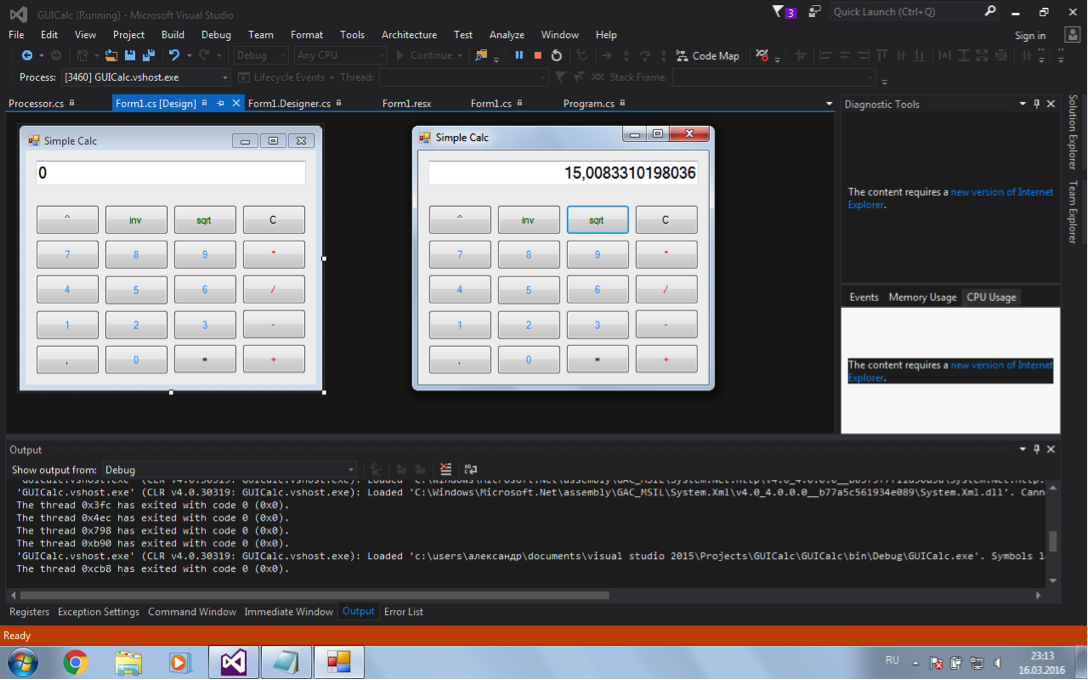
\includegraphics[width=12.5cm]{images/1}
\section*{Concluzii}
In cadrul acestei lucrari de laborator am creat simplu calculator GUI prin intermediul IDE Visual Studio 2015 in limbajul C\#. Calculatorul suporta operatiile simple: +,-,*,/,putere,radical,InversareSemn(+/-), operatii cu numere zecimale. Produsul soft realizat poate fi executat nu doar sub Windows, dar si sub alte platforme (Linux, Mac) în cazul în care este instalat Mono Framework, desi  aplicatia este de tip cross-platform. Cunostintele obtinute pe parcursul desfasurarii lucrarii de laborator vor fi utile pentru realizarea proiectelor ce urmeaza.
\section*{Bibliografie}
\begin{enumerate}
\item https://msdn.microsoft.com/ru-ru/library/67ef8sbd.aspx - \textbf{C\# Programming}
\end{enumerate}





\end{document}